%====================================================
% User Interface Mockups
%====================================================
\section{User Interface Mockups}
\label{sec:mockups}

Mockups represent the visual design and layout of the AgriGov Market system interfaces. 
They illustrate how users interact with the system and provide a clear vision of the system’s graphical structure before implementation.

These mockups were designed to ensure usability, efficiency, and accessibility for all actors of the platform.


\subsection{global Interface Structure}
According to \cite{pressman2014}, navigation diagrams are used in user interface design to model the interaction flow between screens and to ensure that users can efficiently access system functionalities. They help designers and stakeholders understand how information and actions are organized within the interface.

In the context of the AgriGov Market platform, navigation diagrams are used to represent the navigation paths available to each actor (farmer, buyer, transporter, and administrator), showing how users access the different services provided by the system.
\begin{figure}[H]
	\hspace{-2.2cm} % adjust this value
	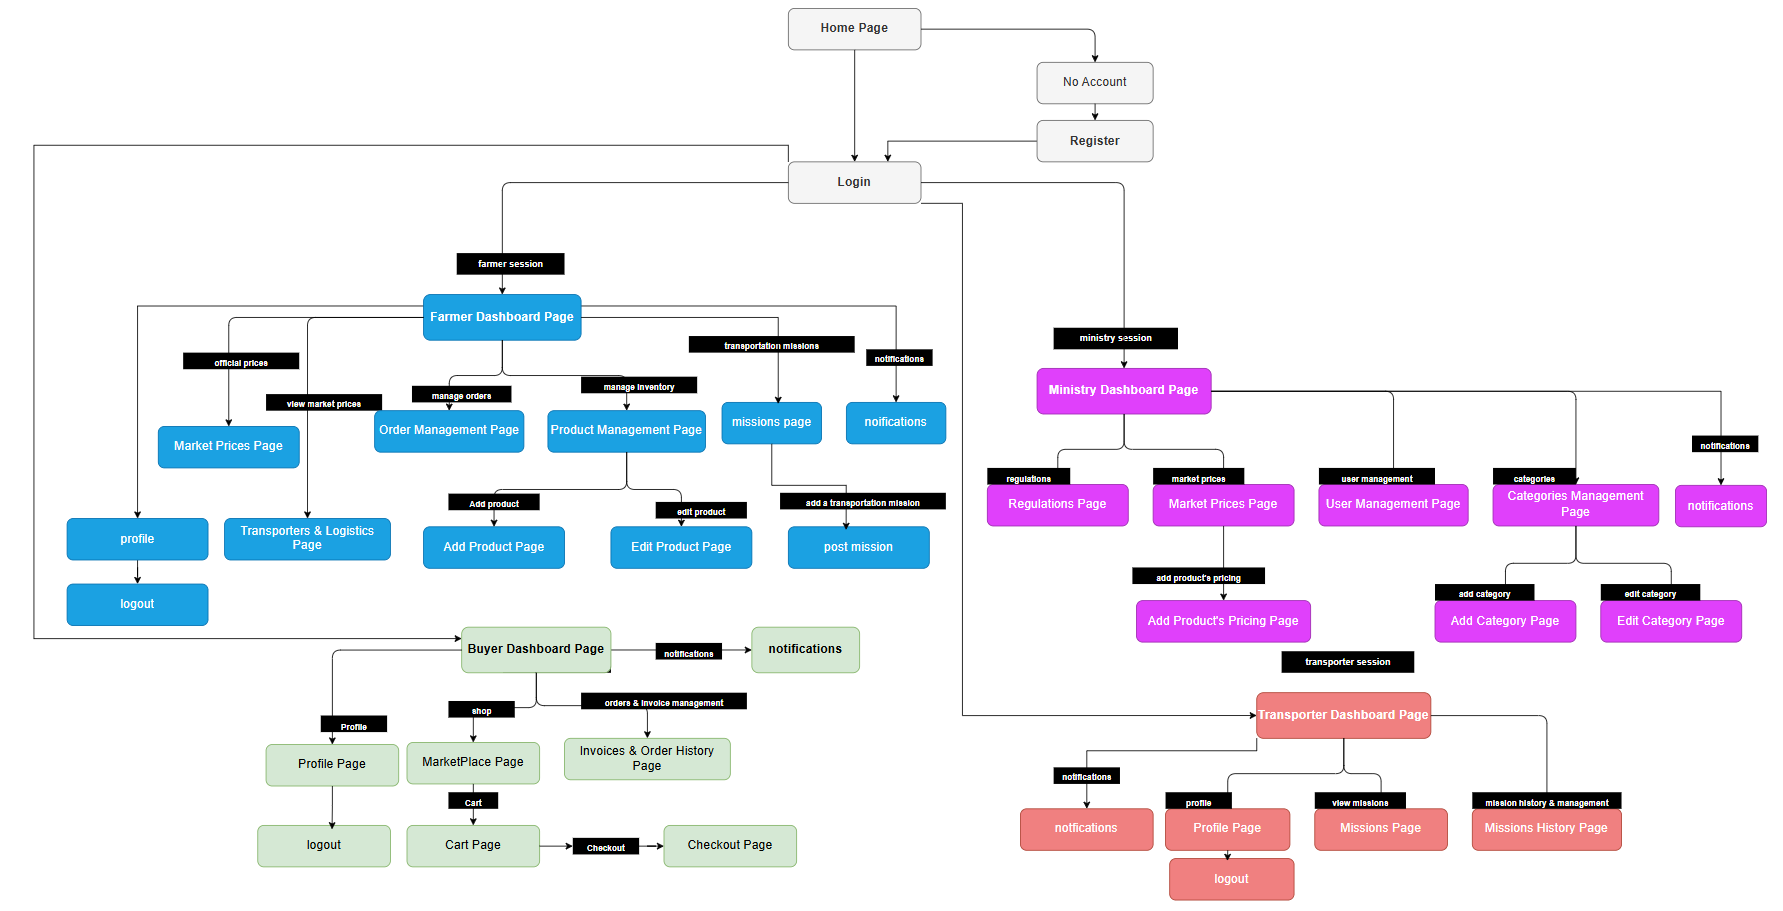
\includegraphics[width=1.3\textwidth]{images/navigation/global-navigation}
	\caption{Global Navigation Diagram}
	\label{fig:global-navigation}
\end{figure}

%----------------------------------------------------
\subsection{Farmer Interface}

A navigation diagram represents the structure and flow of navigation between the different user interfaces of a system. It illustrates how users move from one screen to another and highlights the relationships between the various pages or functionalities of the application. 


\begin{figure}[H]
	\centering
	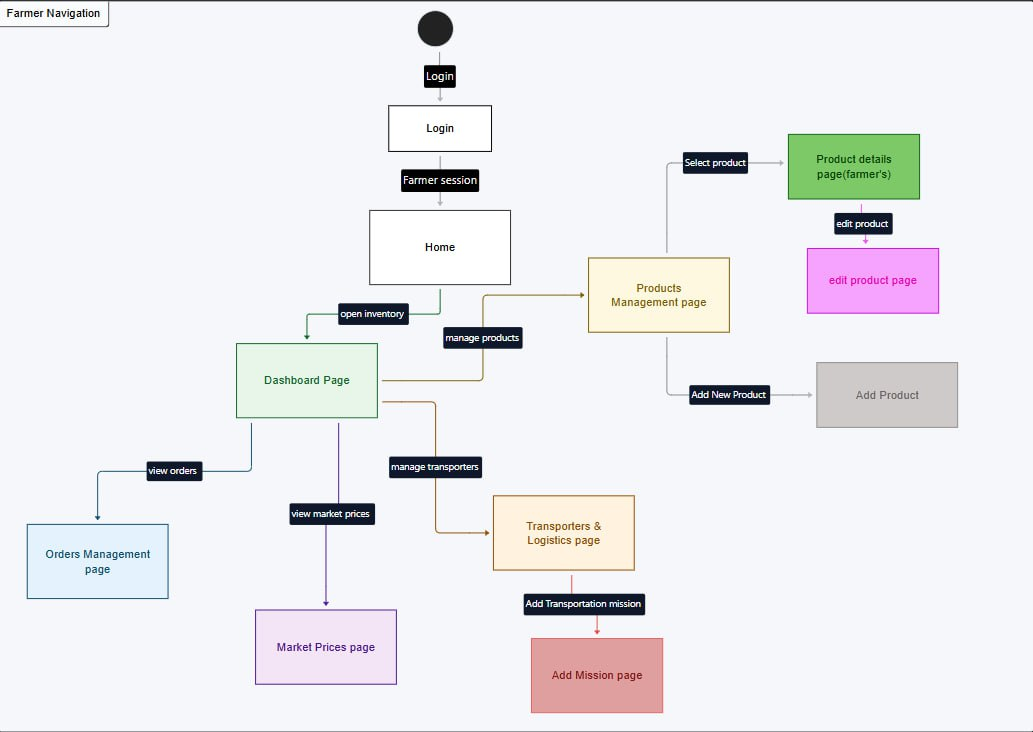
\includegraphics[width=0.9\textwidth]{images/navigation/farmer-navigation}
	\caption{Farmer Navigation Diagram}
	\label{fig:farmer-navigation}
\end{figure}
\begin{figure}[H]
	\centering

% Row 1
\begin{subfigure}[b]{0.45\textwidth}
	\centering
	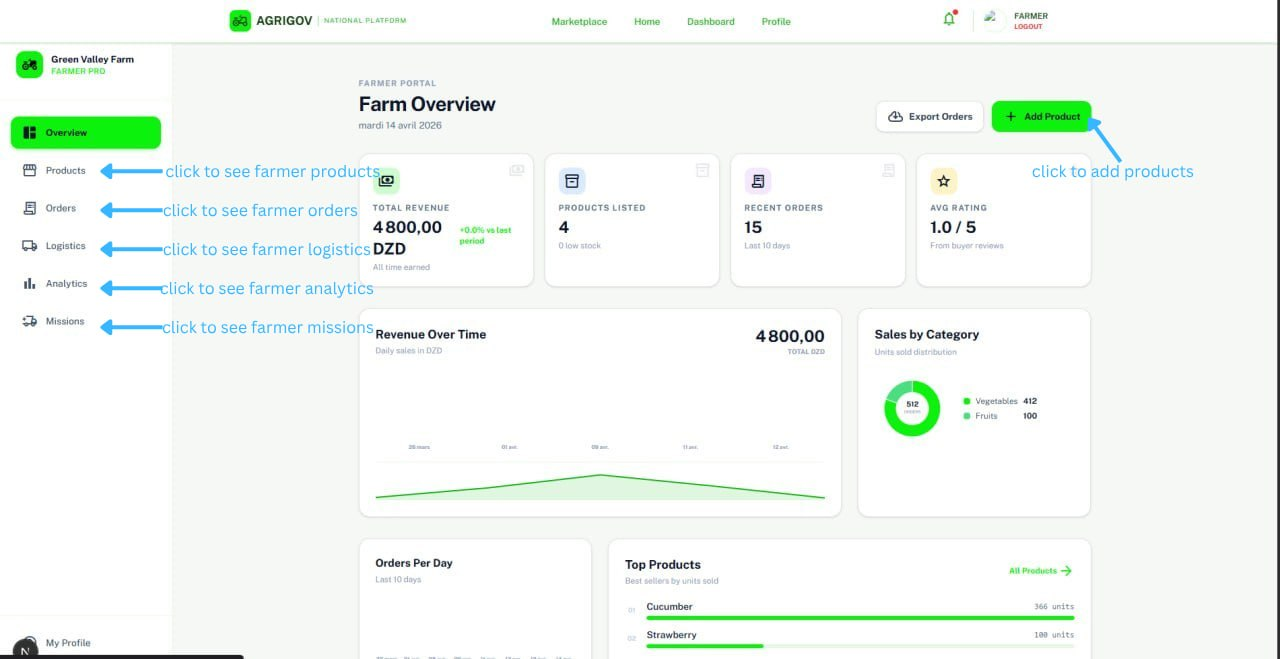
\includegraphics[width=\textwidth]{images/figma/farmer/Overview}
	\caption{Overview Page}
\end{subfigure}
\hfill
\begin{subfigure}[b]{0.45\textwidth}
	\centering
	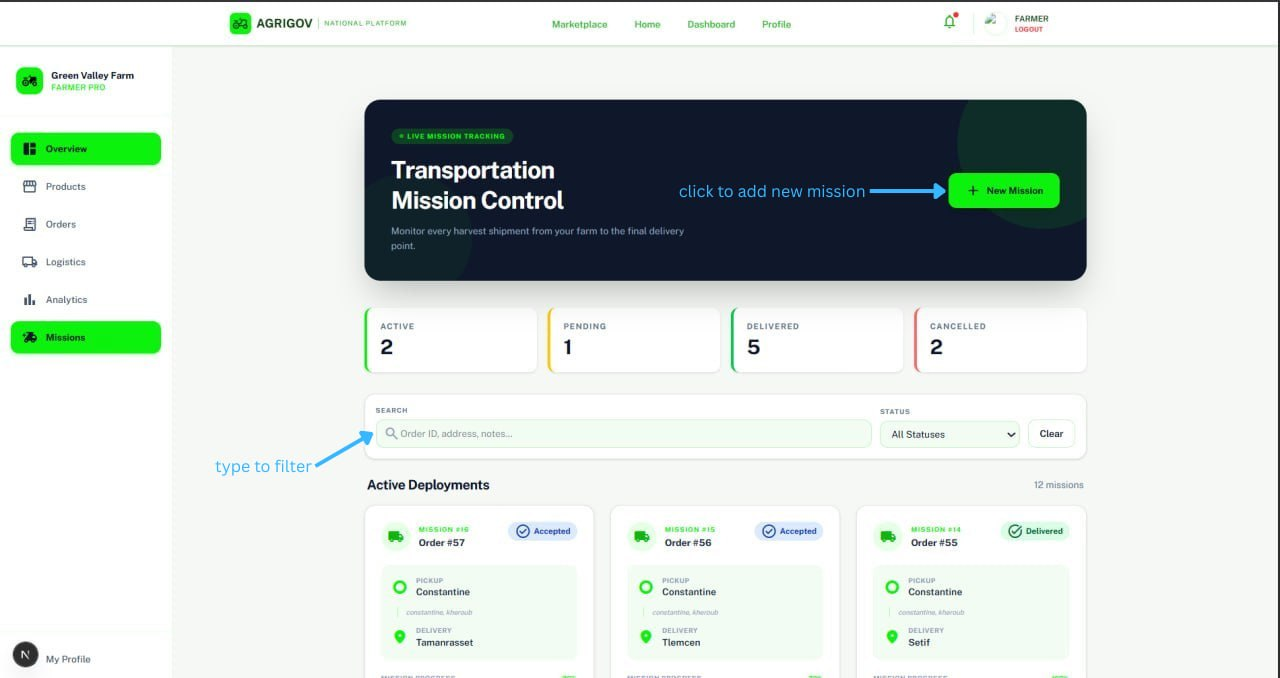
\includegraphics[width=\textwidth]{images/figma/farmer/Transportation mission control}
	\caption{Transportation mission control}
\end{subfigure}

\vspace{0.5cm}
\end{figure}
\begin{figure}[H]
	\centering
	
	% Row 1
	\begin{subfigure}[b]{0.45\textwidth}
		\centering
		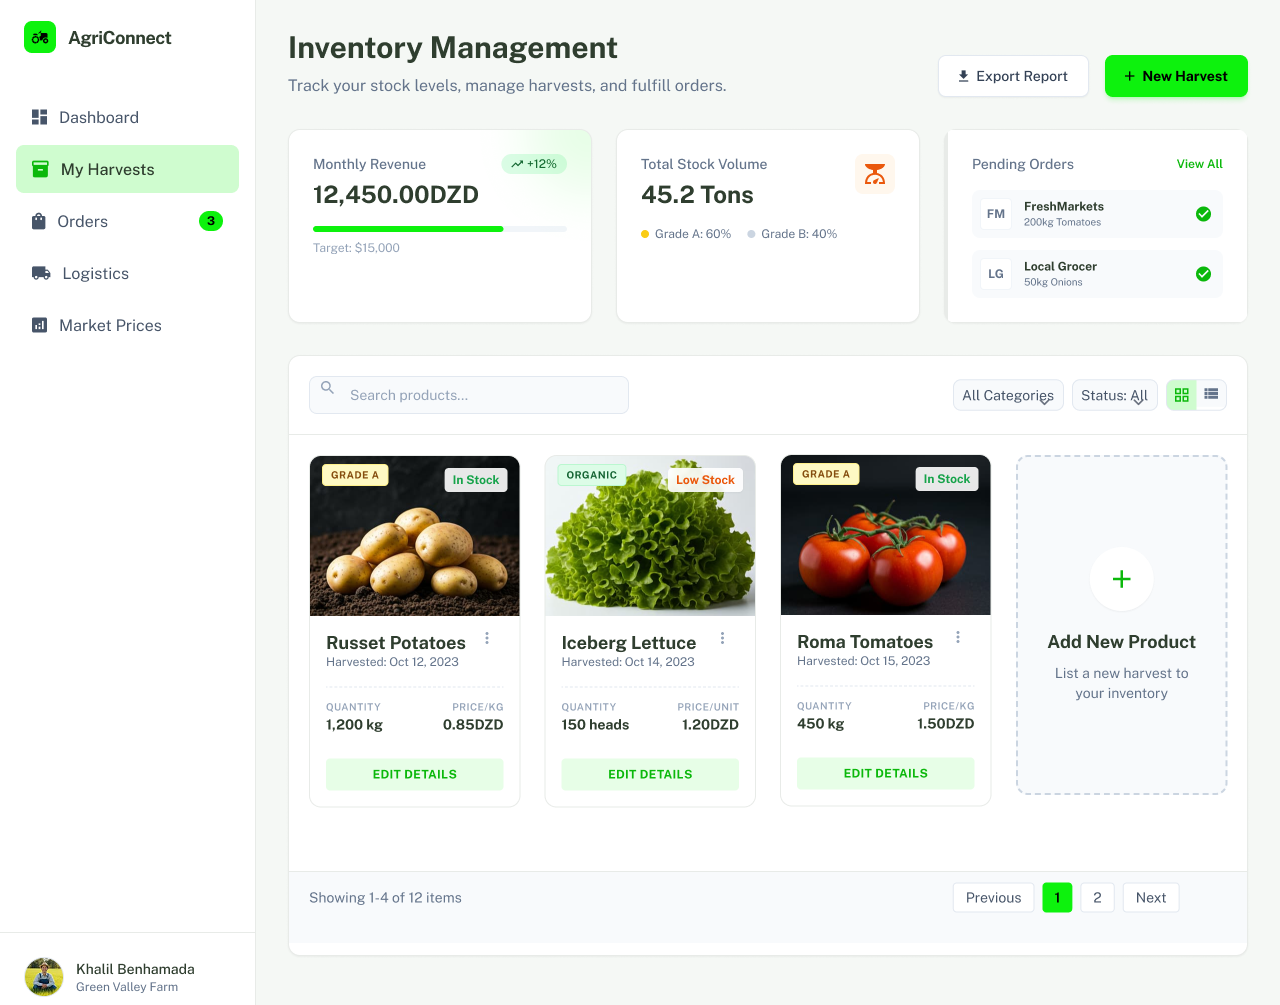
\includegraphics[width=\textwidth]{images/figma/farmer/Farmer Inventory Management}
		\caption{Farmer Inventory Management}
	\end{subfigure}
	\hfill
	\begin{subfigure}[b]{0.45\textwidth}
		\centering
		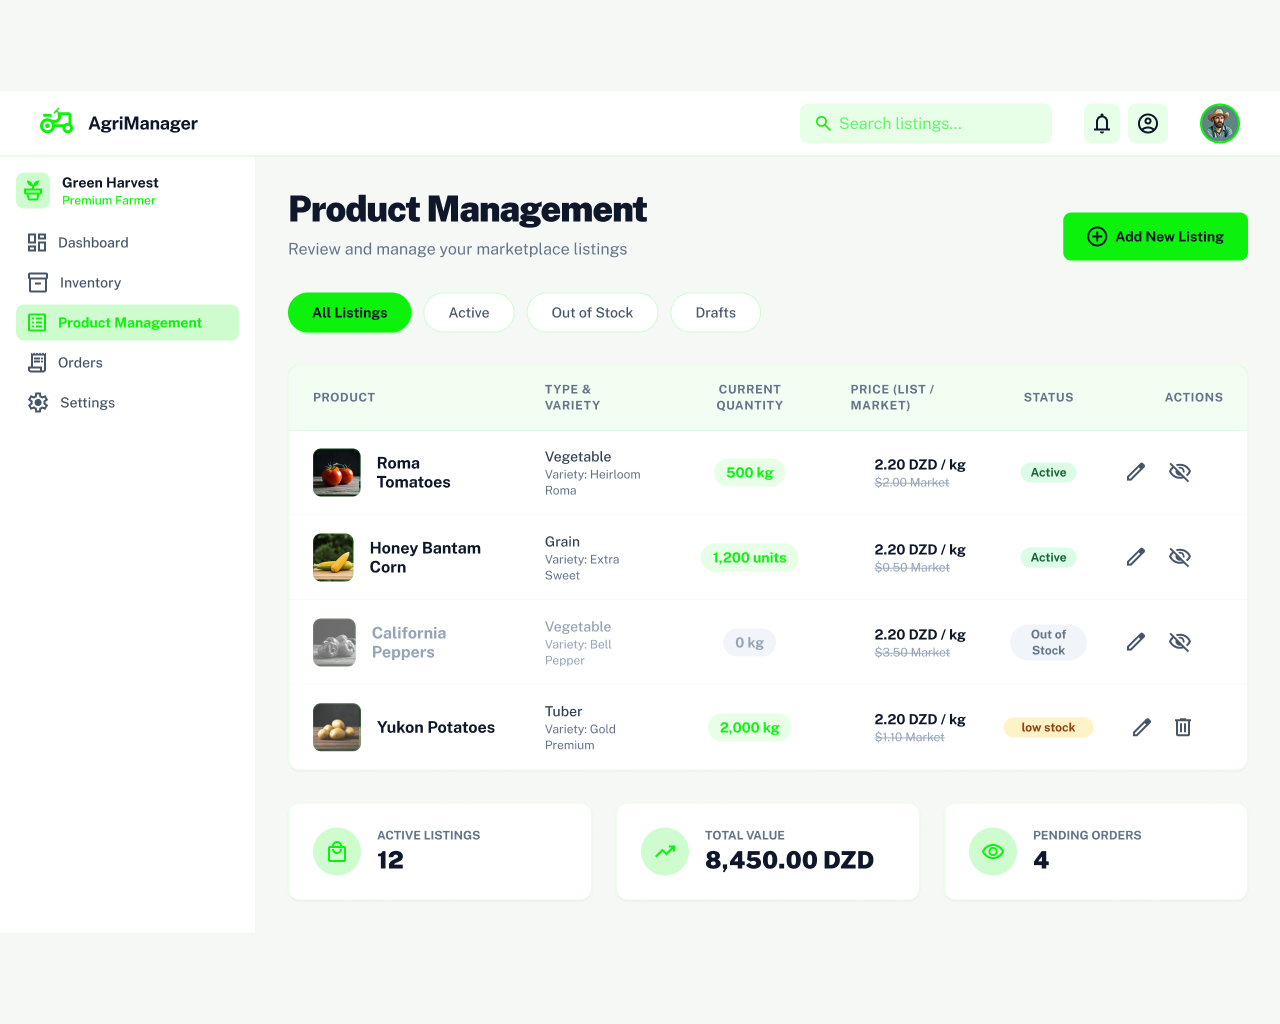
\includegraphics[width=\textwidth]{images/figma/farmer/Product Management}
		\caption{Add New Product}
	\end{subfigure}
	
	\vspace{0.5cm}
	
	% Row 2
	
	\hfill
	
	% Mobile stacked in same column
	\begin{subfigure}[b]{0.95\textwidth}
		\centering
		\begin{subfigure}[b]{0.45\textwidth}
			\centering
			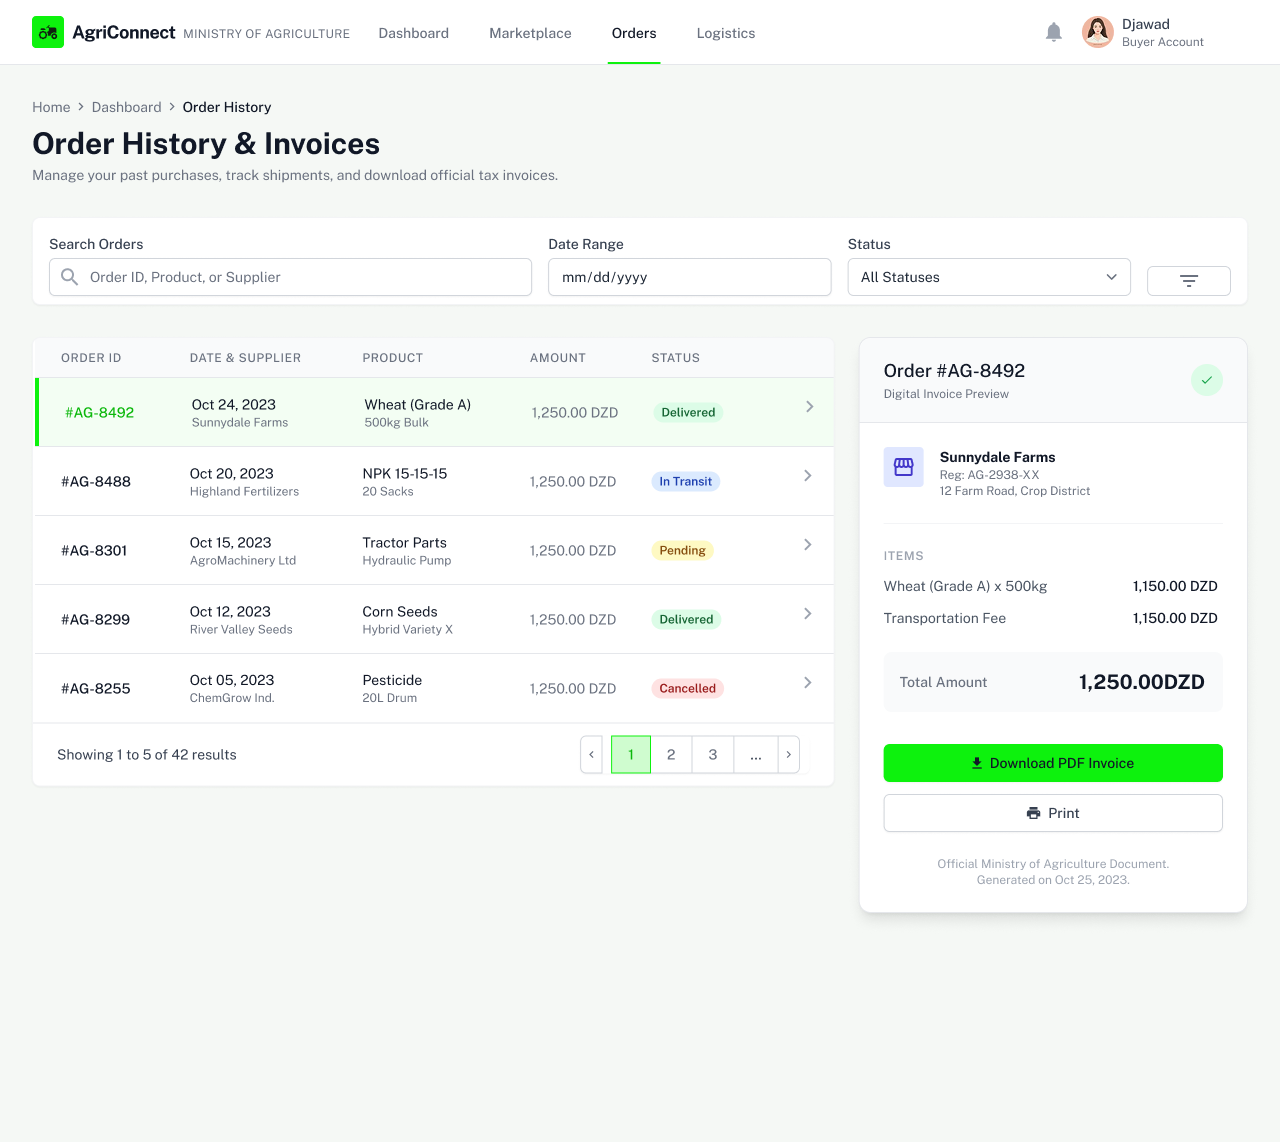
\includegraphics[width=\textwidth]{images/figma/farmer/Order History and Invoices}
			\caption{Order History and Invoices}
		\end{subfigure}
		\hfill
			% Mobile stacked in same column
		\begin{subfigure}[b]{0.17\textwidth}
			\centering
			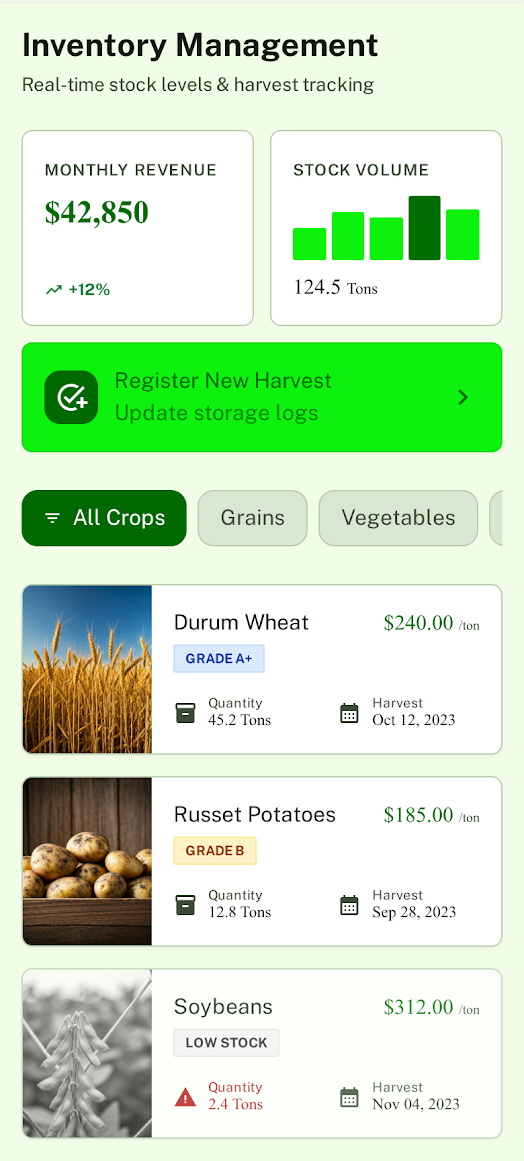
\includegraphics[width=\textwidth]{images/mobile/exports/inventorymanagement}
			\caption{Mobile Login}
		\end{subfigure}
		\hfill
		\begin{subfigure}[b]{0.17\textwidth}
			\centering
			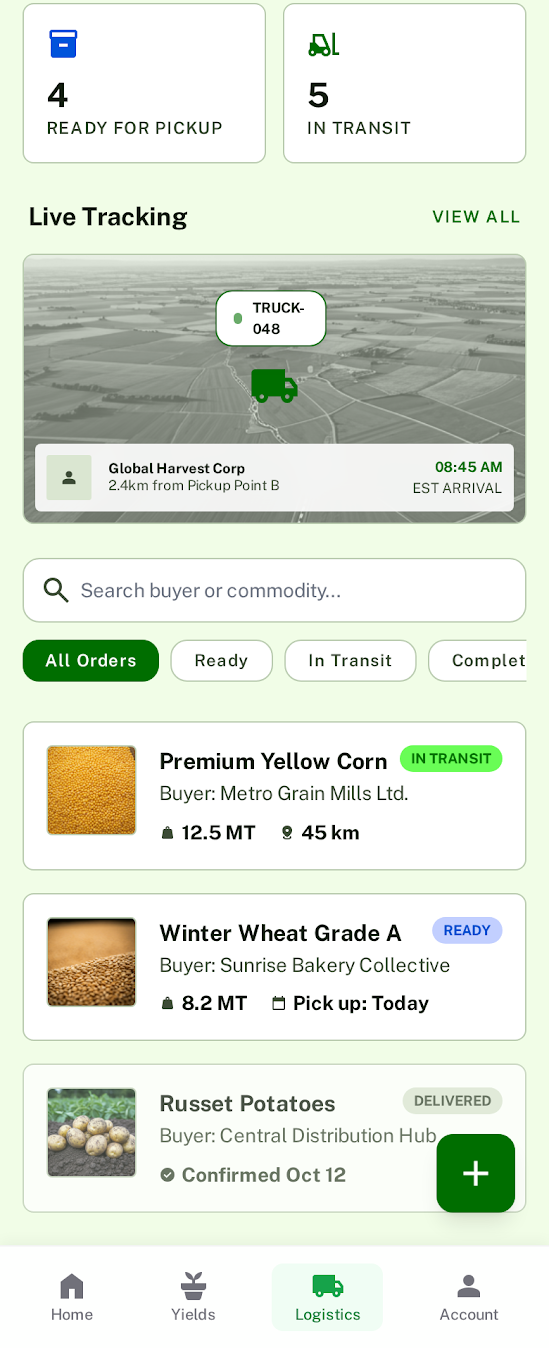
\includegraphics[width=\textwidth]{images/mobile/exports/logistics}
			\caption{Mobile Registration}
		\end{subfigure}
		\hfill
		\begin{subfigure}[b]{0.17\textwidth}
			\centering
			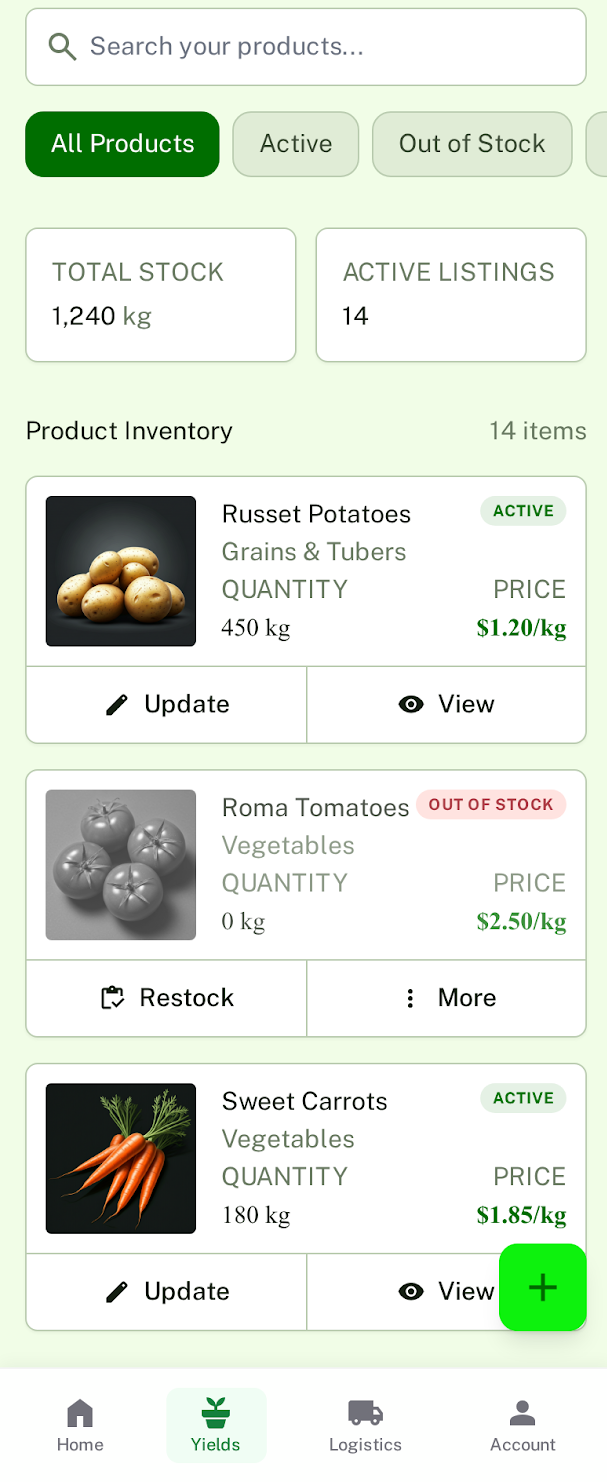
\includegraphics[width=\textwidth]{images/mobile/exports/productManagement}
			\caption{Mobile Registration}
		\end{subfigure}
		
	\end{subfigure}
	
	\caption{Farmer Interface Mockups}
	\label{fig:farmer-ui}
\end{figure}

%----------------------------------------------------
\subsection{Buyer Interface}
\begin{figure}[H]
	\centering
	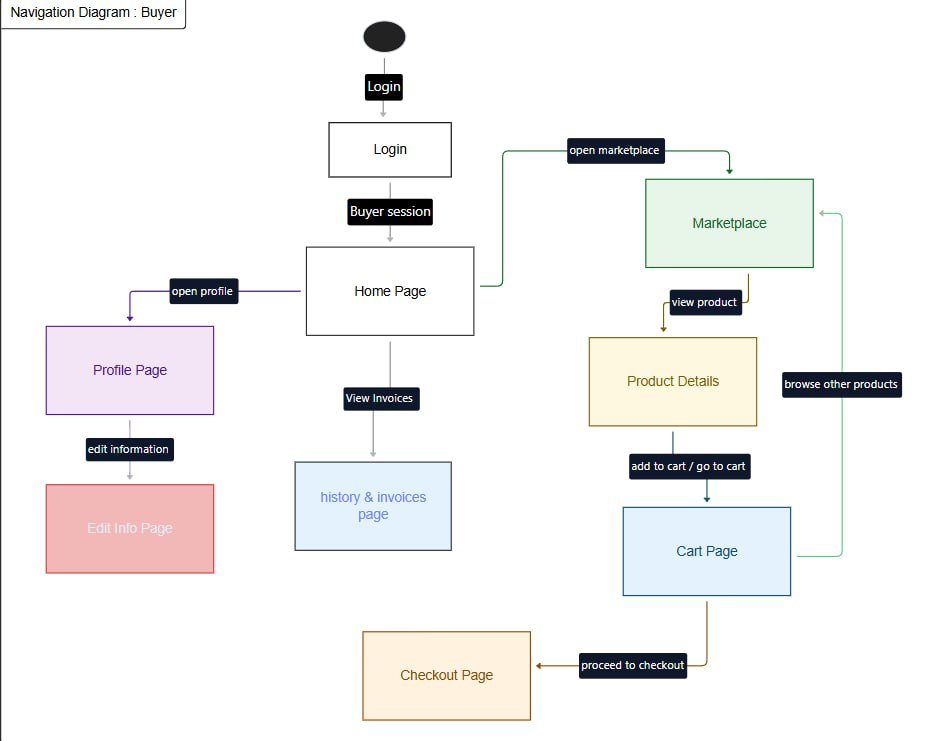
\includegraphics[width=0.9\textwidth]{images/navigation/buyer-navigation}
	\caption{Buyer Navigation Diagram}
	\label{fig:buyer-navigation}
\end{figure}
\begin{figure}[H]
	\centering
	\begin{subfigure}[b]{0.45\textwidth}
		\centering
		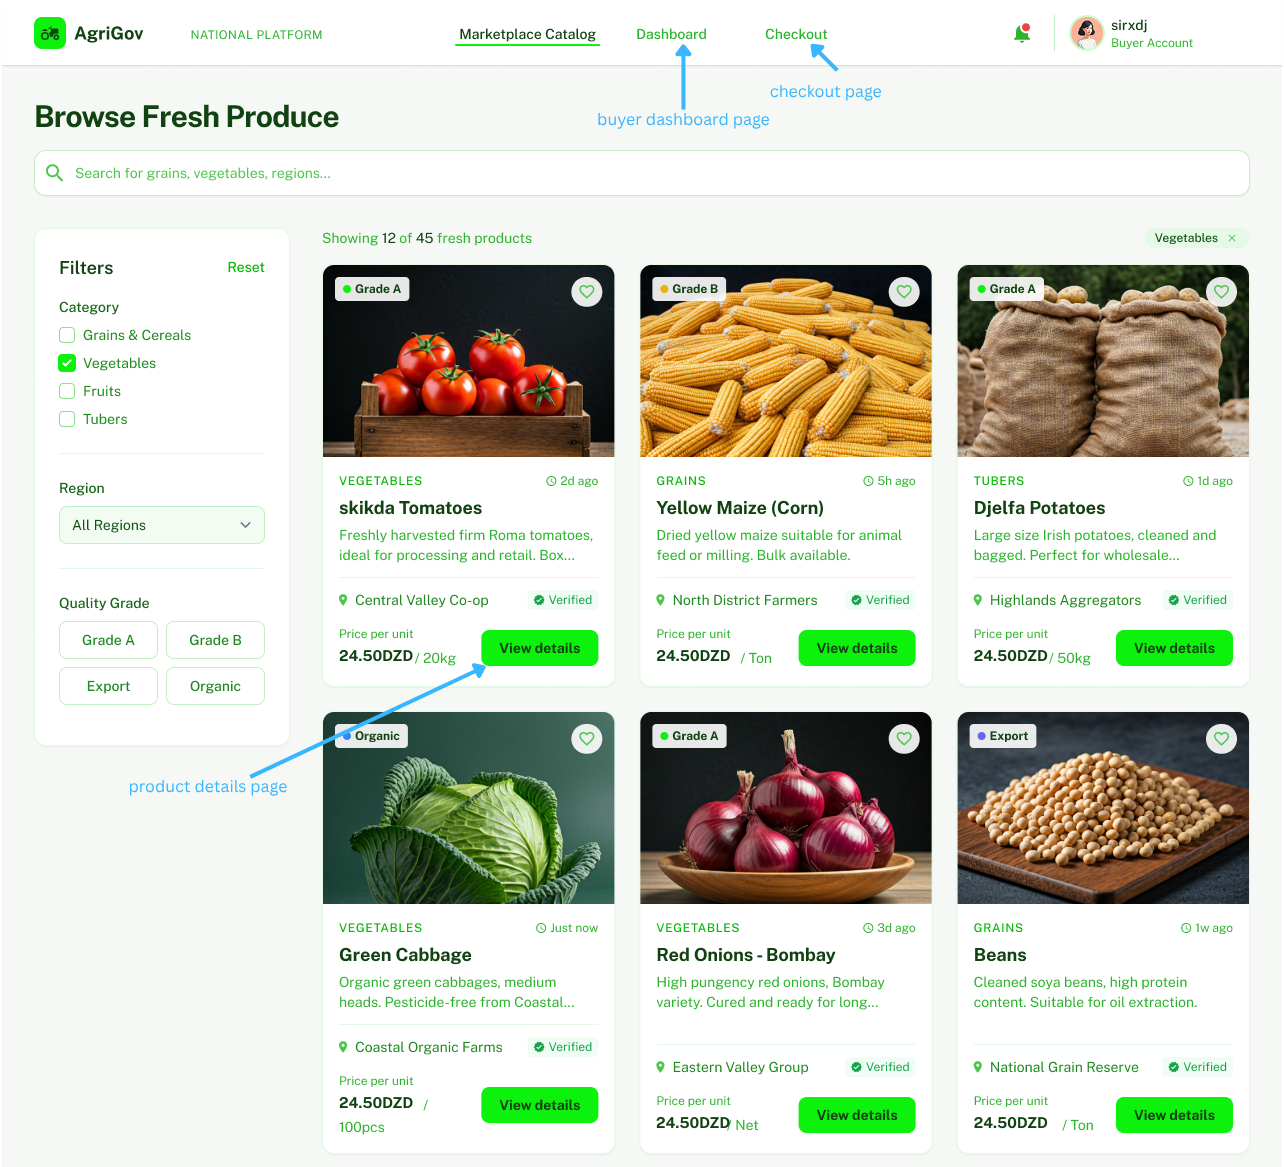
\includegraphics[width=\textwidth]{images/figma/buyer/Buyer Marketplace Catalog}
		\caption{Marketplace Product Catalog}
	\end{subfigure}
	\hfill
	\begin{subfigure}[b]{0.45\textwidth}
		\centering
		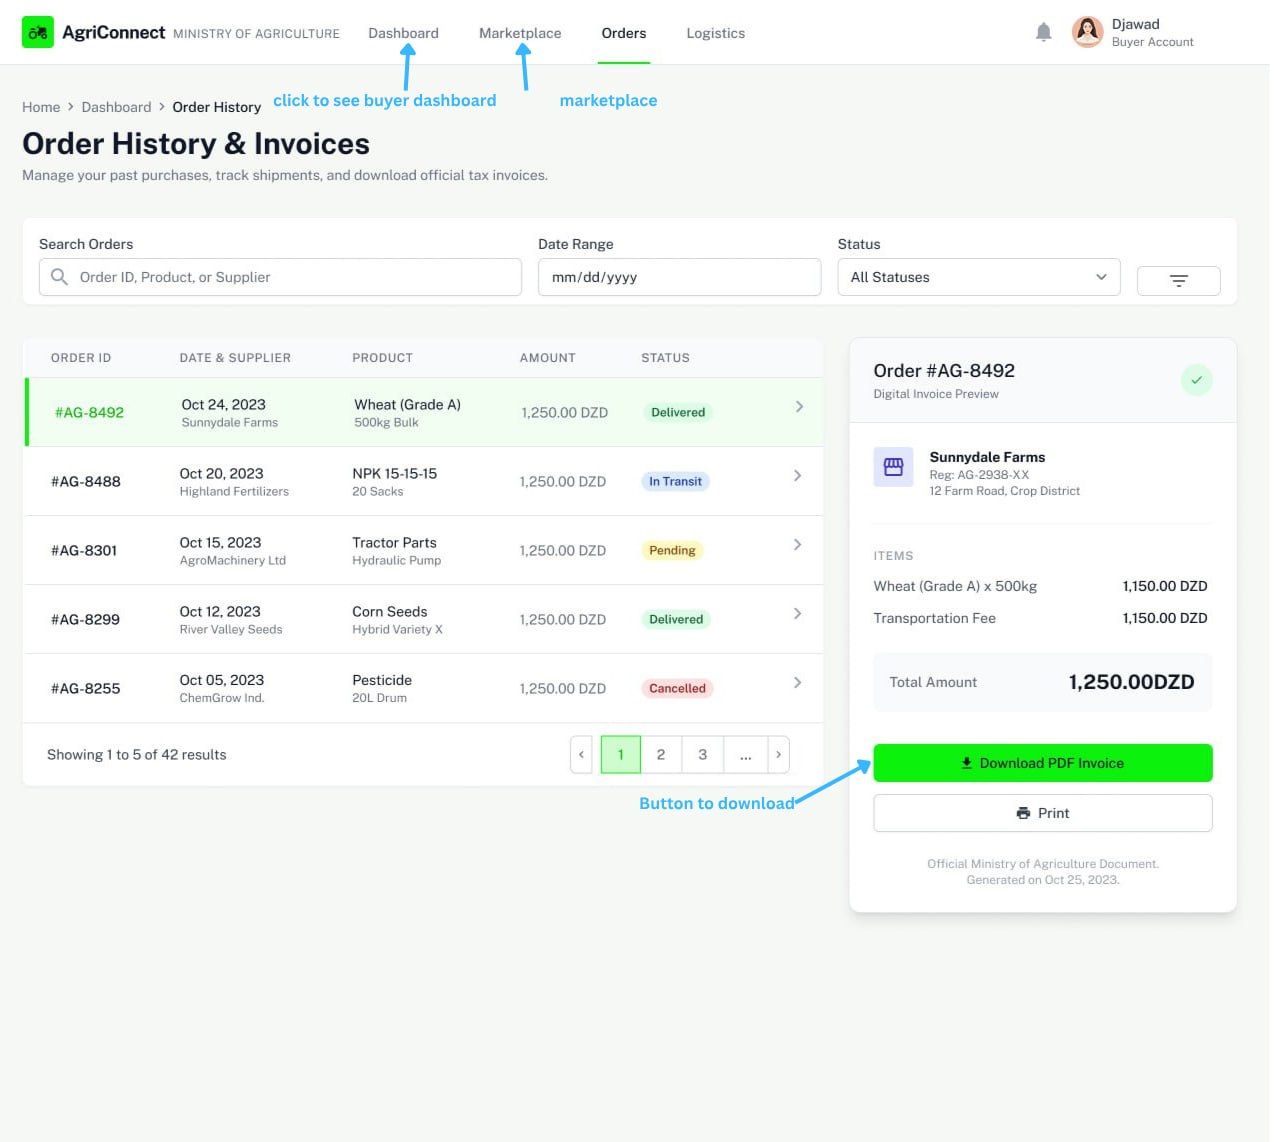
\includegraphics[width=\textwidth]{images/figma/buyer/order history}
		\caption{Buyer Order History}
	\end{subfigure}
	
	\vspace{0.5cm}
\end{figure}
\begin{figure}[H]
	\centering
	
	
	
	\begin{subfigure}[b]{0.45\textwidth}
		\centering
		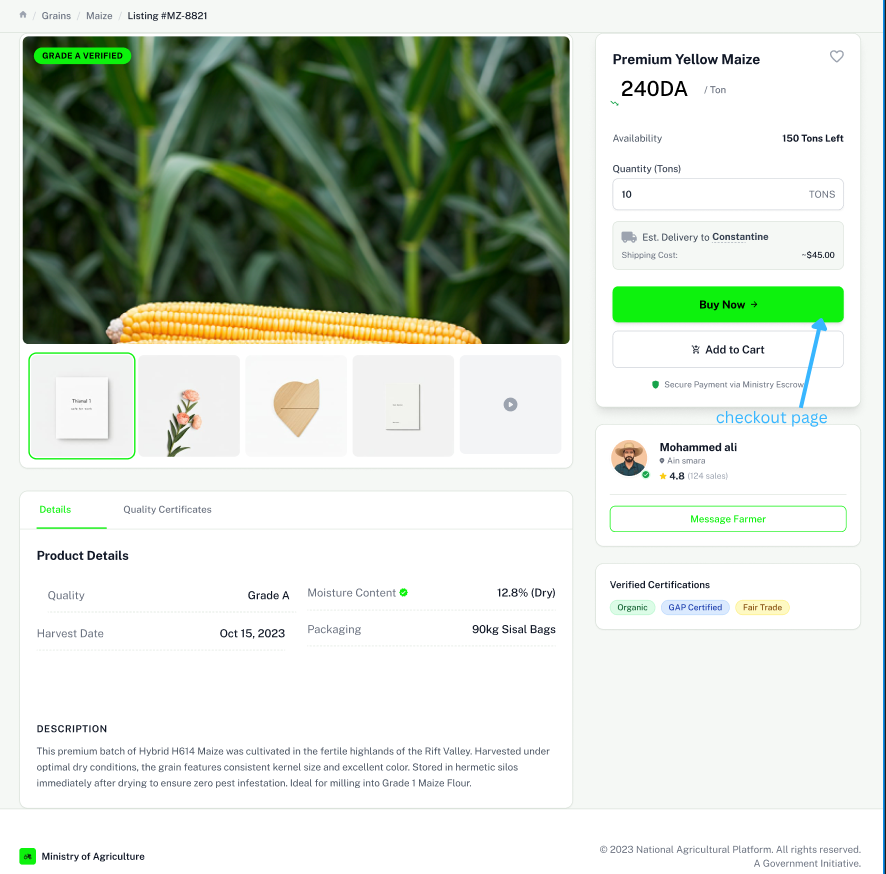
\includegraphics[width=\textwidth]{images/figma/buyer/Product Specification Details}
		\caption{Product Specification Details}
	\end{subfigure}
	\hfill
	\begin{subfigure}[b]{0.17\textwidth}
		\centering
		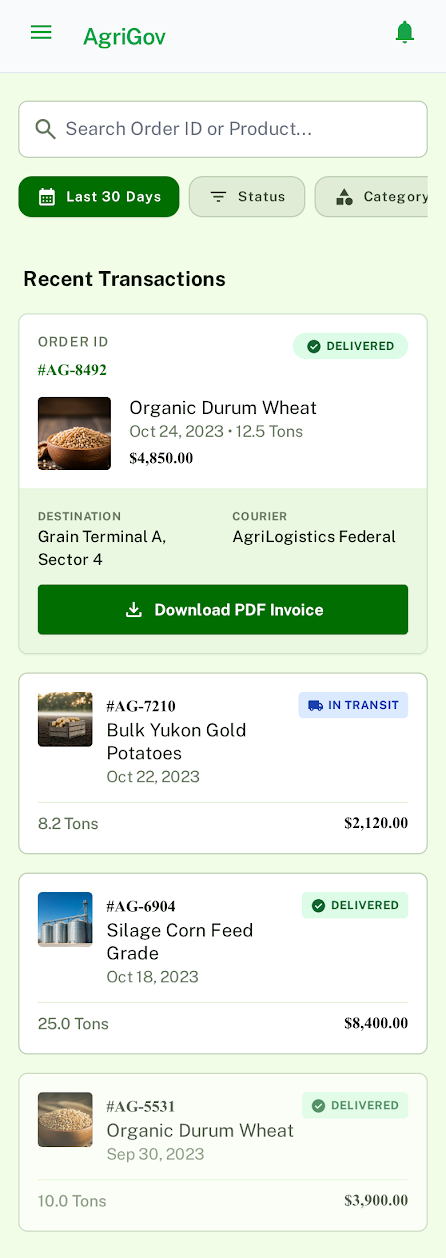
\includegraphics[width=\textwidth]{images/mobile/exports/orderhistory}
		\caption{Order History mobile}
	\end{subfigure}
	\begin{subfigure}[b]{0.17\textwidth}
		\centering
		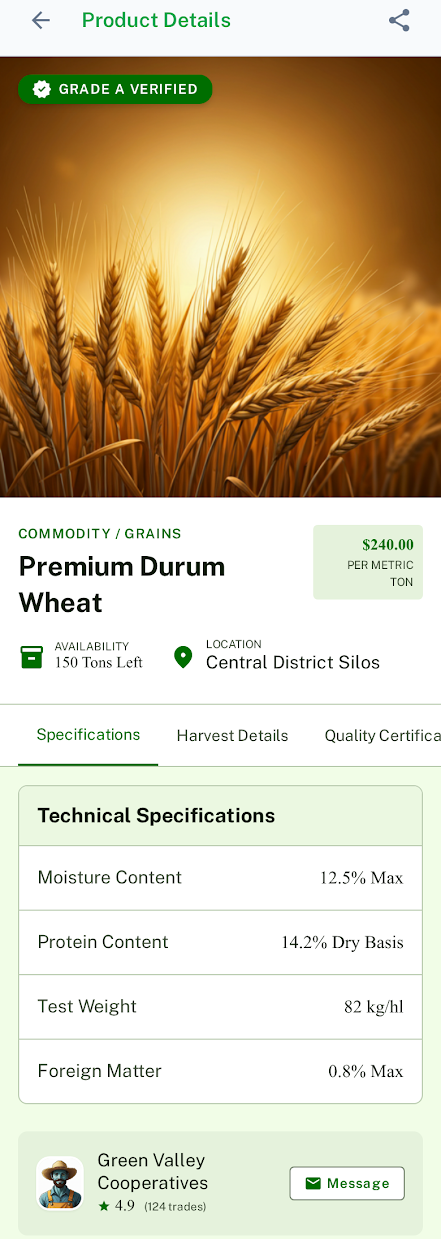
\includegraphics[width=\textwidth]{images/mobile/exports/productdetail}
		\caption{Product detail mobile}
	\end{subfigure}
	\begin{subfigure}[b]{0.17\textwidth}
		\centering
		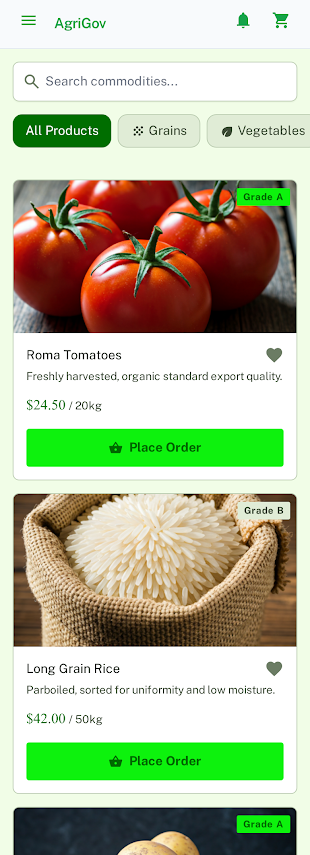
\includegraphics[width=\textwidth]{images/mobile/exports/catalog}
		\caption{Catalogue mobile}
	\end{subfigure}
	
	\caption{Buyer Interface Mockups}
	\label{fig:buyer-ui}
	
\end{figure}

%----------------------------------------------------
\subsection{Transporter Interface}
\begin{figure}[H]
	\centering
	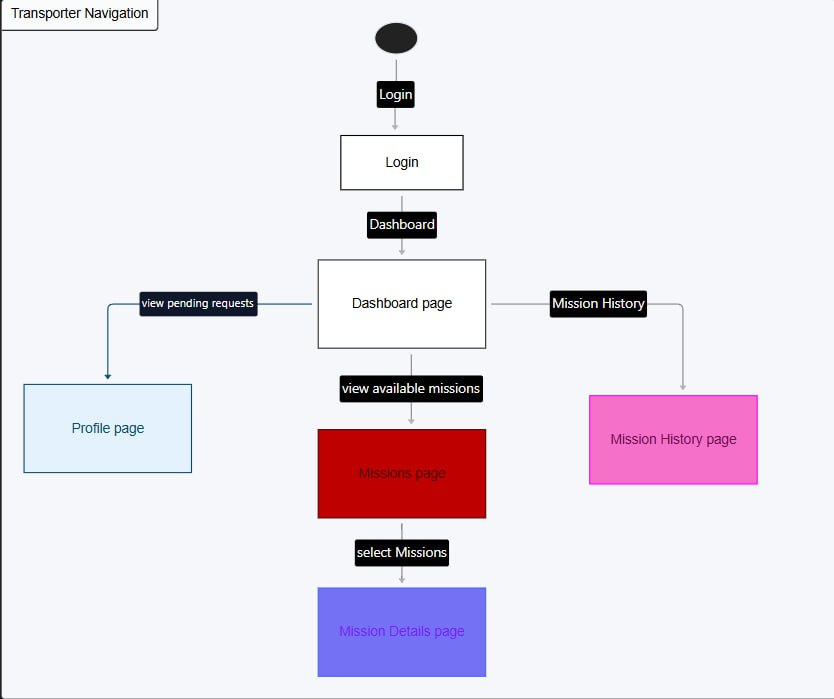
\includegraphics[width=0.9\textwidth]{images/navigation/transporter-navigation}
	\caption{Transporter Navigation Diagram}
	\label{fig:transporter-navigation}
\end{figure}
\begin{figure}[H]
	\centering
	
	\begin{subfigure}[b]{0.45\textwidth}
		\centering
		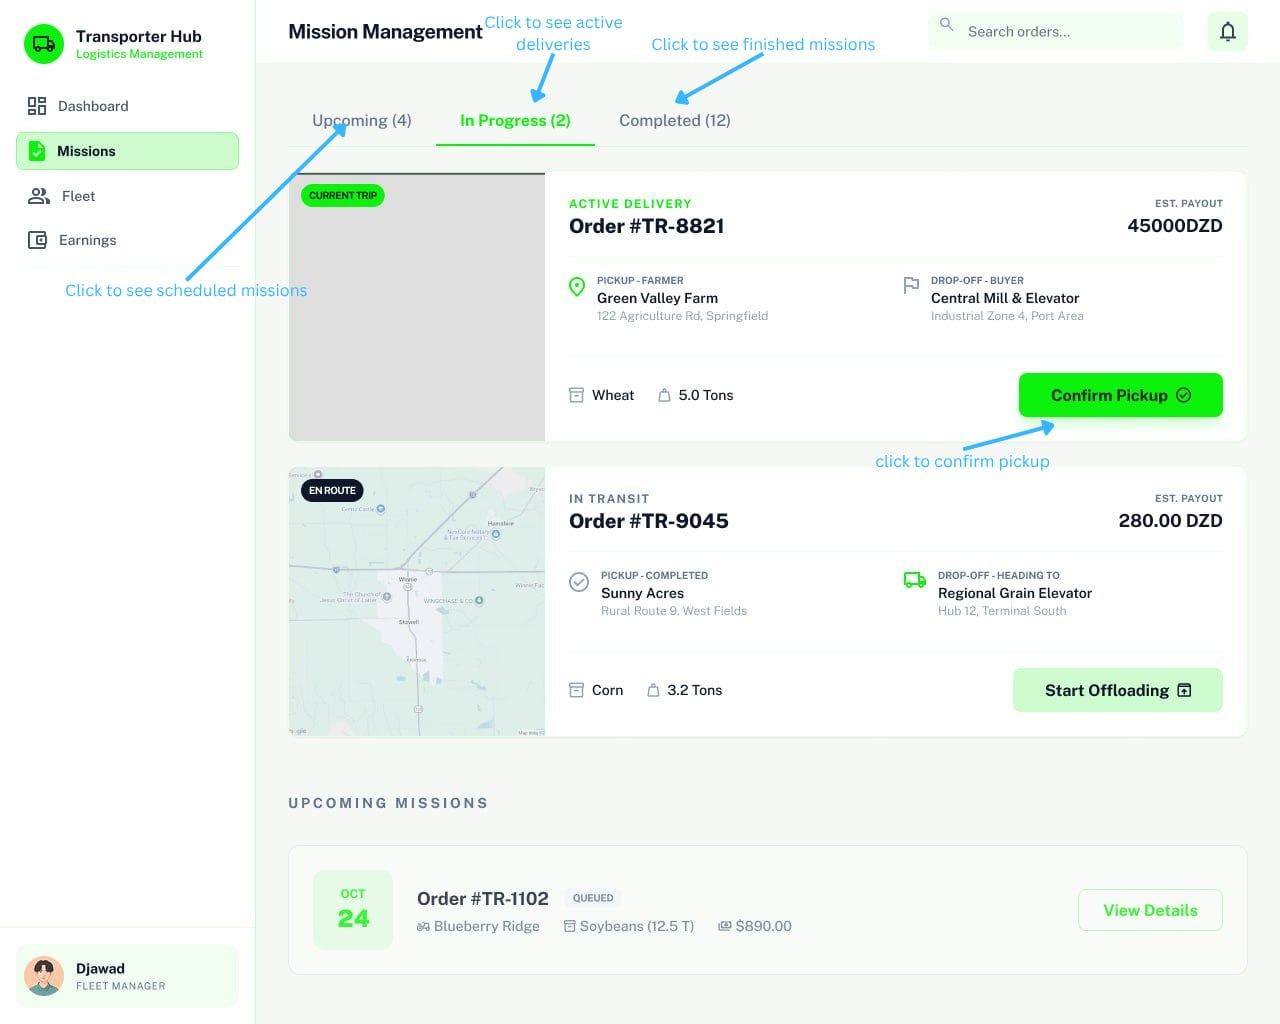
\includegraphics[width=\textwidth]{images/figma/transporter/Body-1}
		\caption{Transporter Dashboard}
	\end{subfigure}
	\hfill
	\begin{subfigure}[b]{0.45\textwidth}
		\centering
		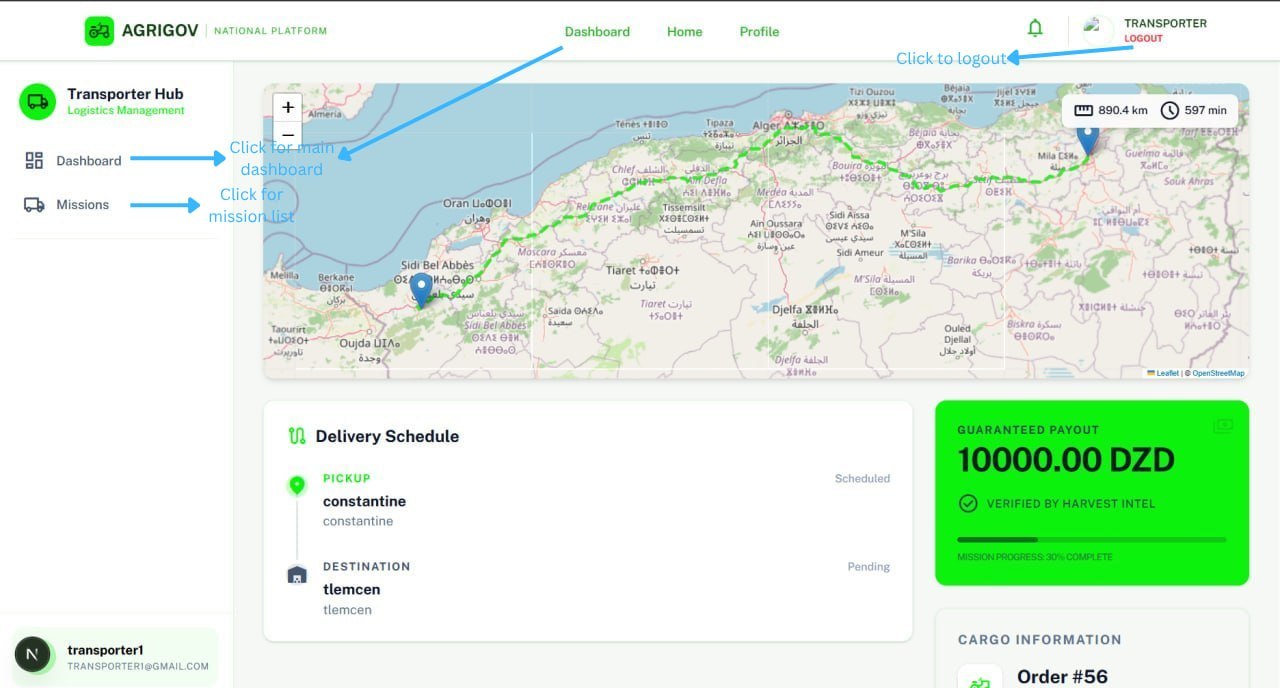
\includegraphics[width=\textwidth]{images/figma/transporter/Transporter Mission Control}
		\caption{Transporter Mission Control}
	\end{subfigure}
	
	
	
	
\end{figure}
\begin{figure}[H]
	\centering
	
	
	
	\begin{subfigure}[b]{0.17\textwidth}
		\centering
		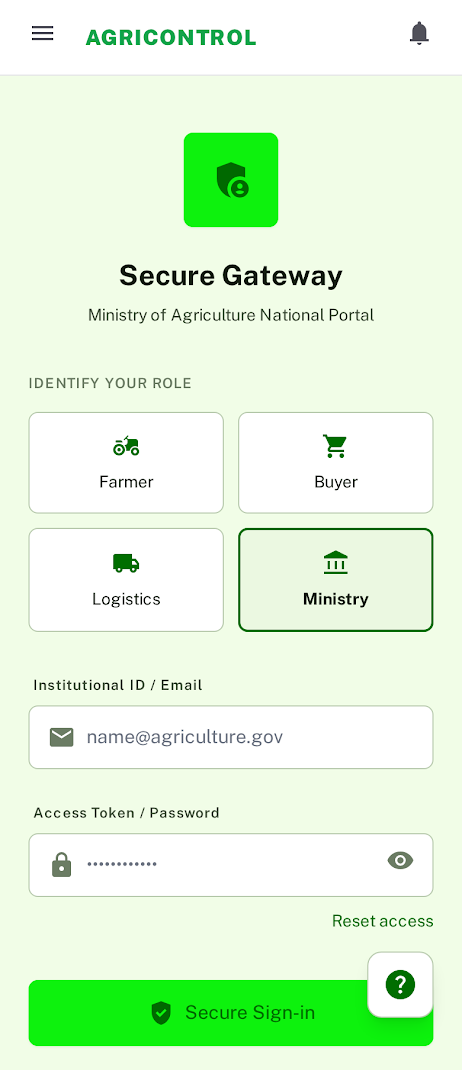
\includegraphics[width=\textwidth]{images/mobile/exports/login}
		\caption{mobile login}
	\end{subfigure}
	\hfill
	\begin{subfigure}[b]{0.17\textwidth}
		\centering
		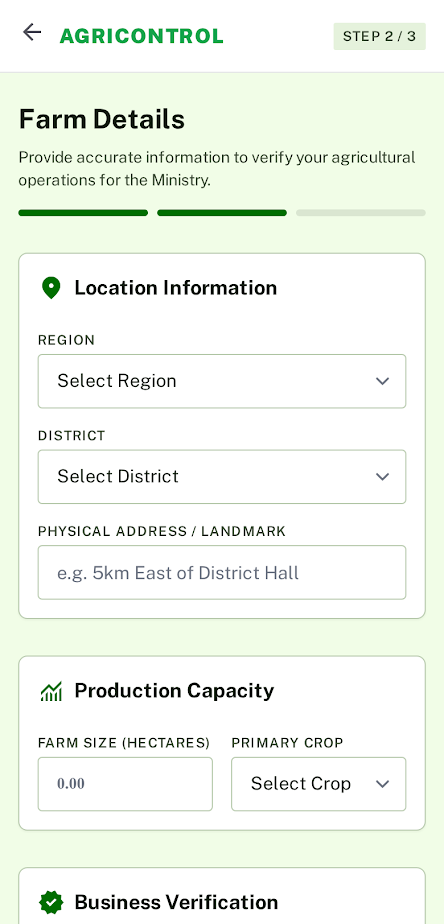
\includegraphics[width=\textwidth]{images/mobile/exports/registration}
		\caption{registration mobile}
	\end{subfigure}
		\hfill
	\begin{subfigure}[b]{0.17\textwidth}
		\centering
		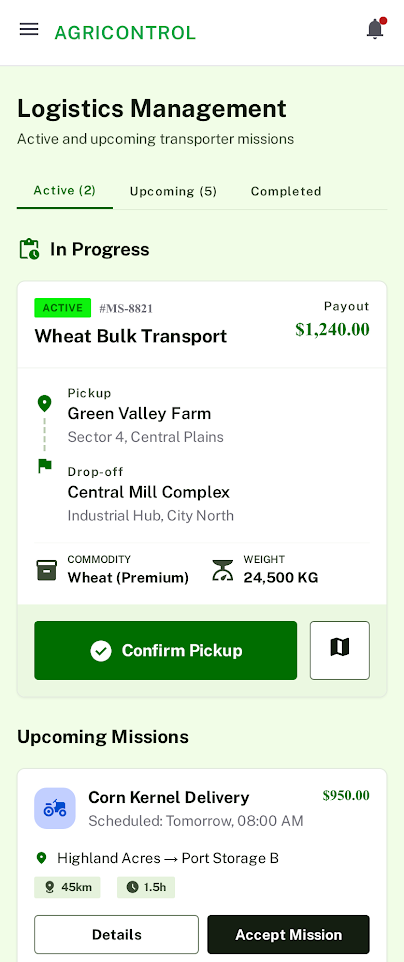
\includegraphics[width=\textwidth]{images/mobile/exports/missions}
		\caption{missions mobile}
	\end{subfigure}
		\hfill
	\begin{subfigure}[b]{0.17\textwidth}
		\centering
		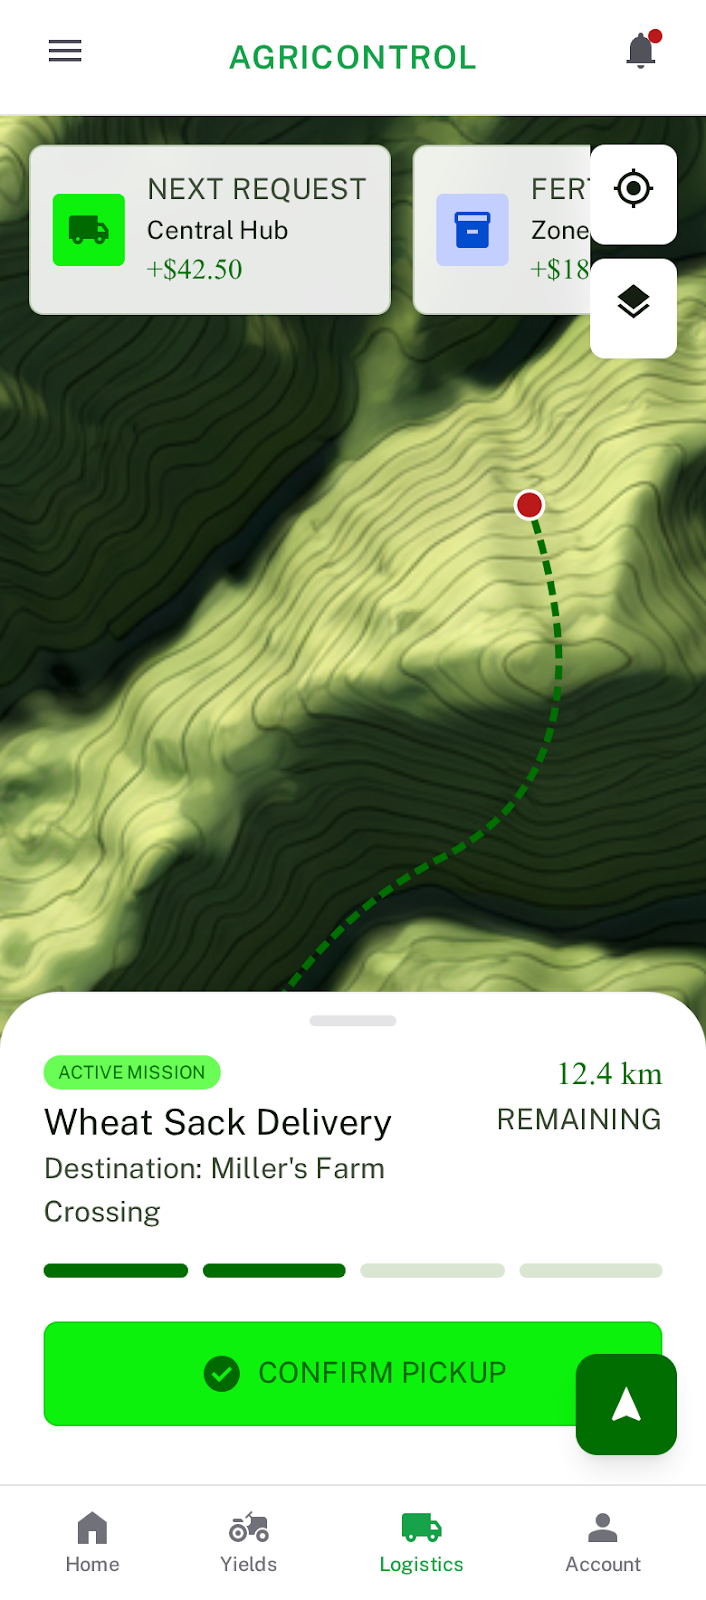
\includegraphics[width=\textwidth]{images/mobile/exports/missioncontrol}
		\caption{mission Controle mobile}
	\end{subfigure}
	
	\caption{Transporter Interface Mockups}
	\label{fig:transporter-ui}
	
\end{figure}

%----------------------------------------------------
\subsection{Ministry Interface}
\begin{figure}[H]
	\centering
	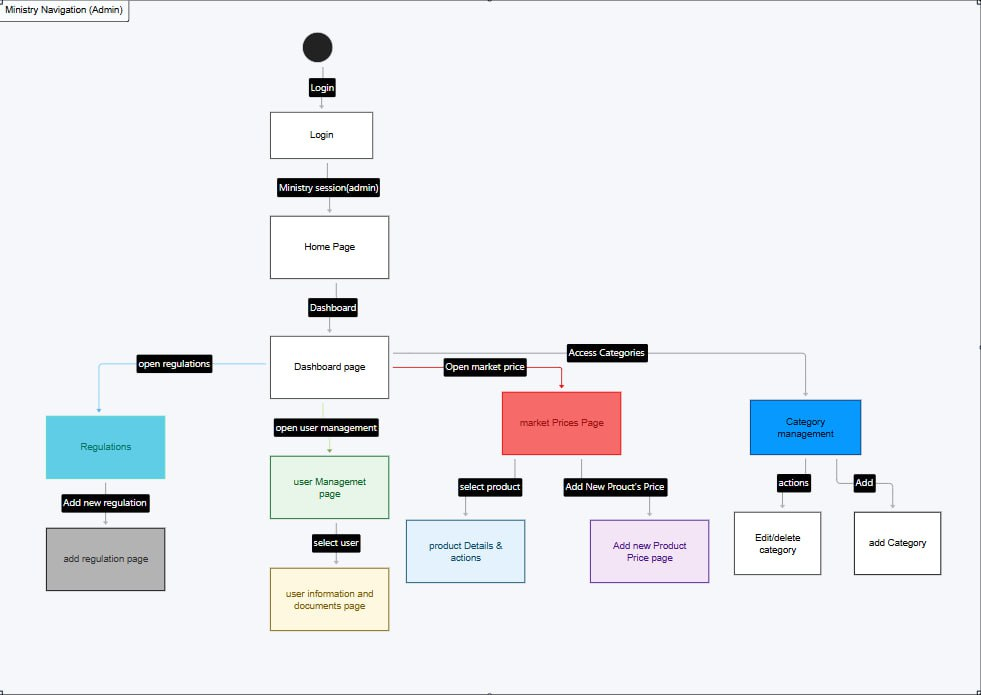
\includegraphics[width=0.9\textwidth]{images/navigation/ministry-navigation}
	\caption{Ministry Navigation Diagram}
	\label{fig:ministry-navigation}
\end{figure}
\begin{figure}[H]
		\centering
	
	\begin{subfigure}[b]{0.45\textwidth}
		\centering
		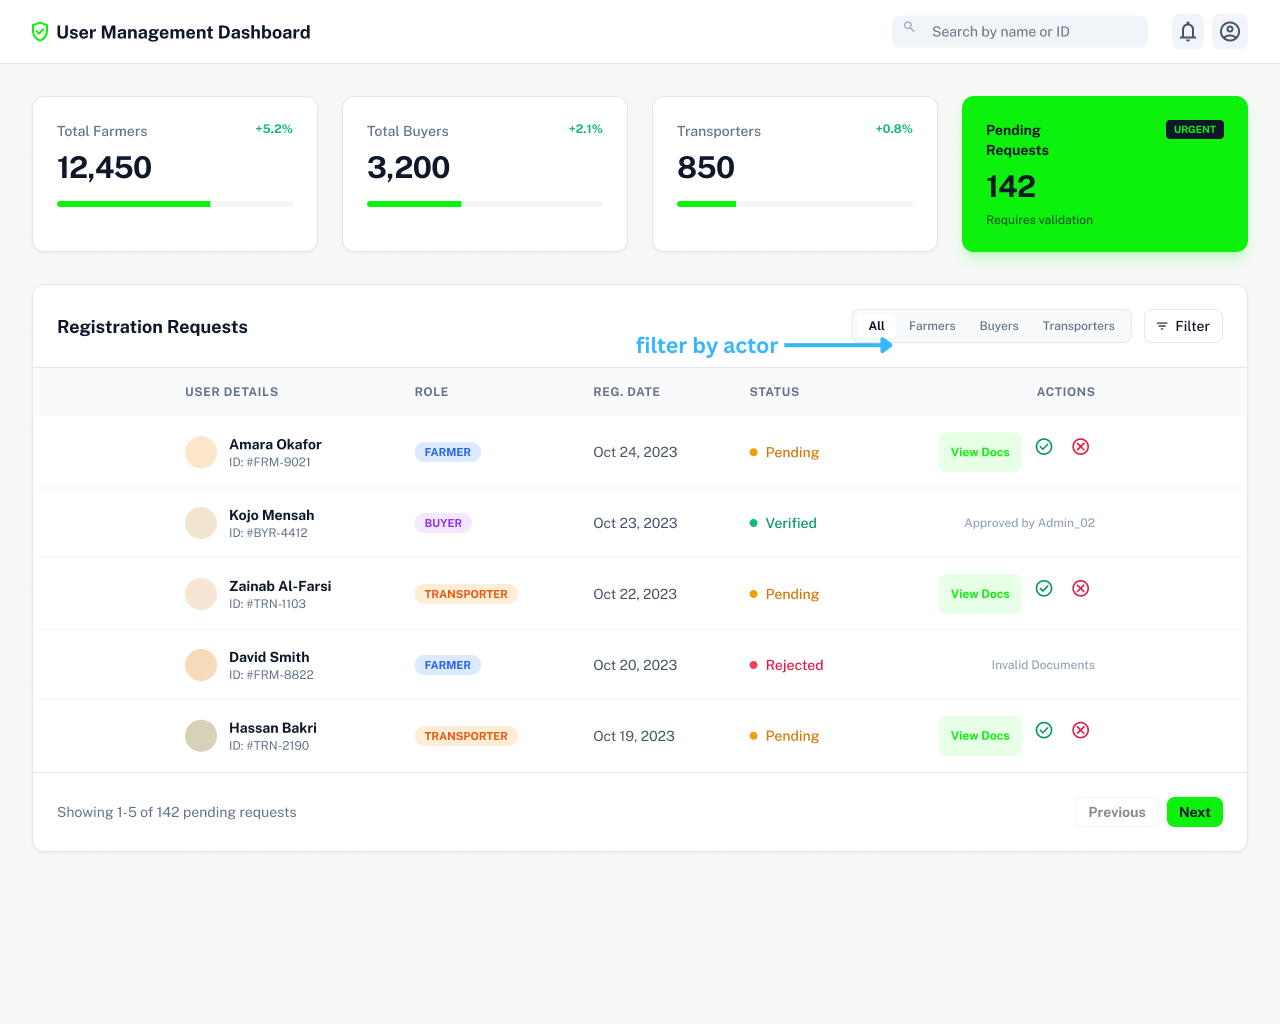
\includegraphics[width=\textwidth]{images/figma/ministry/user management}
		\caption{User Validation Panel}
	\end{subfigure}
	\hfill
	\begin{subfigure}[b]{0.45\textwidth}
		\centering
		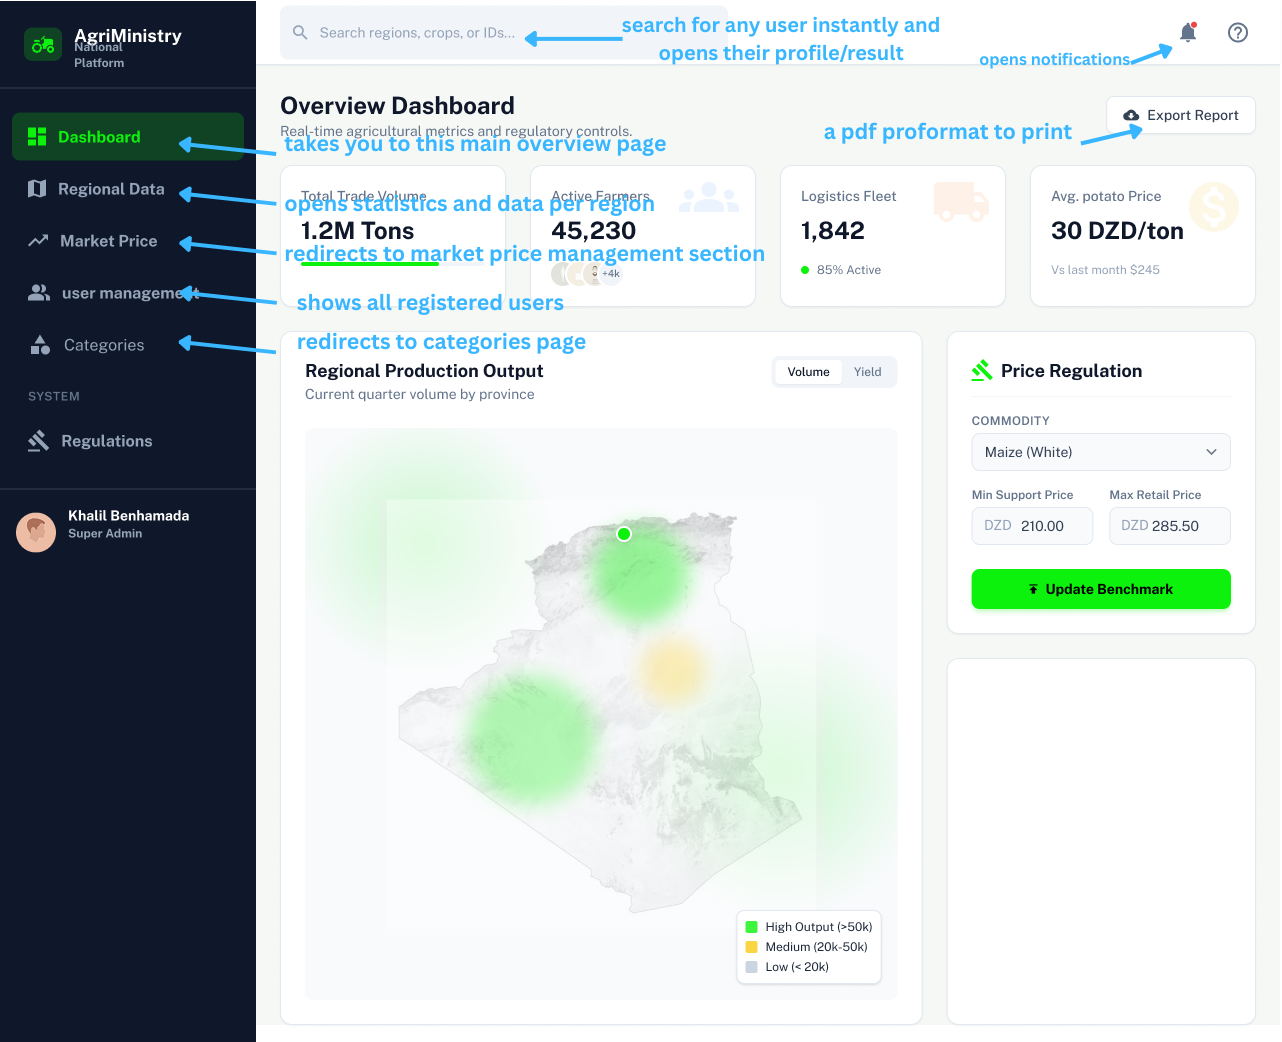
\includegraphics[width=\textwidth]{images/figma/ministry/Ministry Admin Dashboard}
		\caption{Ministry Administration Dashboard}
	\end{subfigure}
	
	\vspace{0.5cm}
\end{figure}
\begin{figure}[H]
	\centering
	
	\begin{subfigure}[b]{0.45\textwidth}
		\centering
		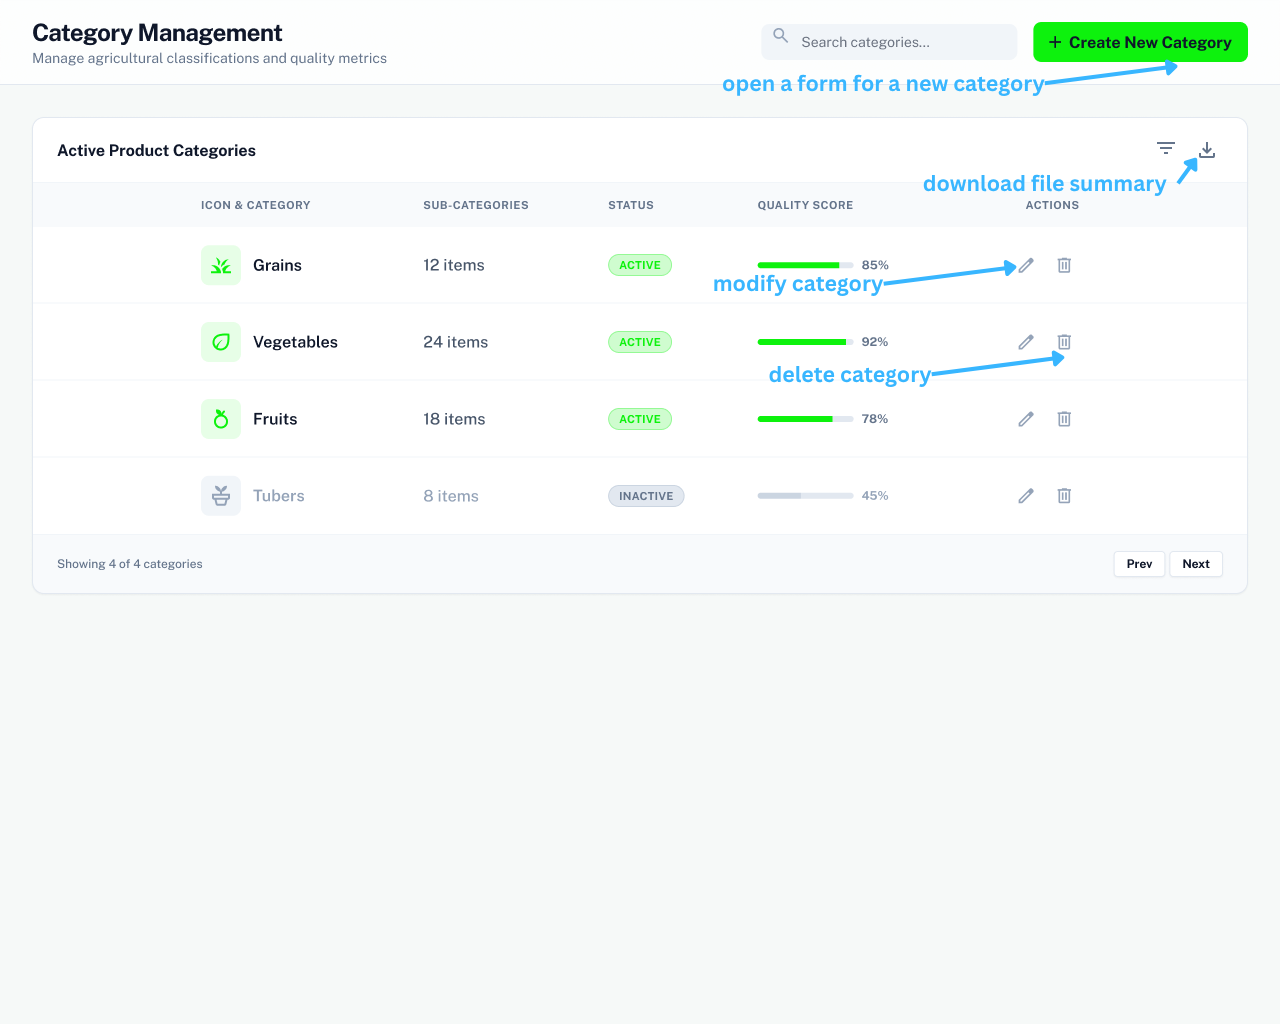
\includegraphics[width=\textwidth]{images/figma/ministry/category}
		\caption{Category management}
	\end{subfigure}
	\hfill
	\begin{subfigure}[b]{0.45\textwidth}
		\centering
		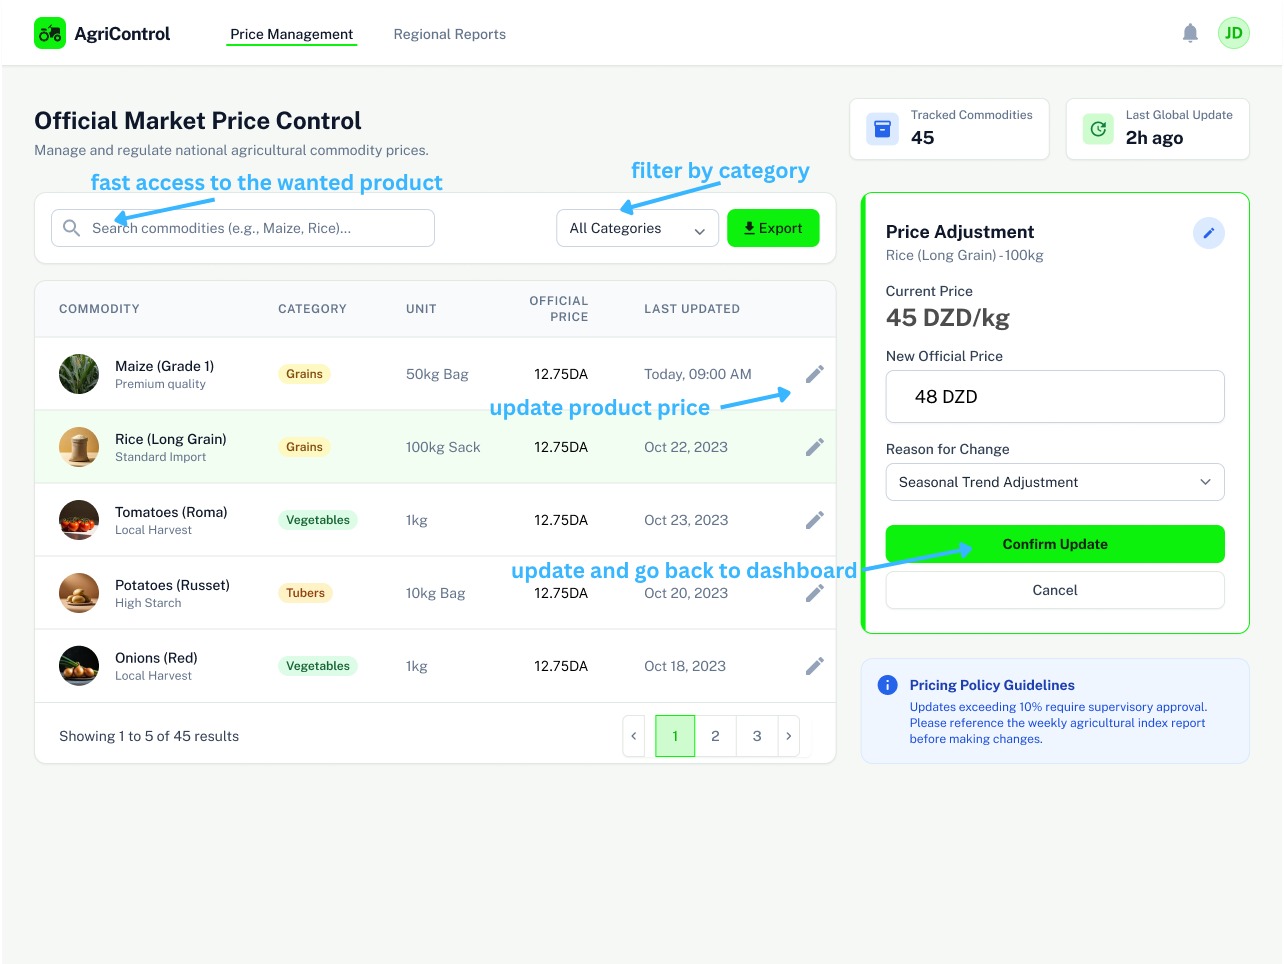
\includegraphics[width=\textwidth]{images/figma/ministry/Official Price Management}
		\caption{Official Price Management}
	\end{subfigure}
	
	\caption{Ministry Interface Mockups}
	\label{fig:ministry-ui}
	
\end{figure}